\documentclass{article}
\usepackage[utf8]{inputenc} % - Defines what coding LaTeX uses. Use this one.
\usepackage[swedish]{babel}
\usepackage{graphicx} % - Package for including images in the document.
\usepackage{amsmath}
\usepackage{mathtools}
\graphicspath{ {Images/} } % - Path to where the images are located on your computer. In this case I have a folder (look to the left) "Images" where the images are gathered.
\usepackage{hyperref} % - Package for including hyperlinks in the document.
\usepackage[backend=bibtex,style=numeric,bibencoding=ascii]{biblatex}
 % - Package for the bibliography ("referenser").
\addbibresource{bibliography.bib} % - From where, i.e. which file, the references are taken. The bibliography file is called name.bib; see left column.
\usepackage{graphicx}
\graphicspath{ {./images/} }
\usepackage{minted}

%%%%%%%%%%%%%%%%%%%%%%%%%%%%%%%%%%%%%%%%%%%%%%%%%%%%%%%%%%%%%%
% -               Title and affiliation                    - %
%%%%%%%%%%%%%%%%%%%%%%%%%%%%%%%%%%%%%%%%%%%%%%%%%%%%%%%%%%%%%%

\title {
	Lab 1
}

\author {
	Philip Wenkel \\
	{\tt phiwen-7@student.ltu.se}
}
% Institutionen för teknikvetenskap och matematik \\ \\
% \includegraphics[width=0.2\textwidth]{ltu_swe.jpg}}
% MG: Bilder på första sidan är bäst att lägga i "author"-
% kommandot såvitt jag kan se.

% Ange författare, e-post samt datum för publiceringen.
% Titelsidan kan också innehålla en figur för att locka läsaren att läsa rapporten.
% Figurens innehåll måste naturligtvis vara kopplat till arbetet som beskrivs i rapporten.
%
% På en titel kan man ställa höga krav. Titeln skall vara klar och beskrivande och fungera
% som en miniatyr-sammanfattning av arbetet. Läsaren skall förstå vad rapporten handlar om
% genom att läsa titeln. Trots det ska titeln vara kort, 4-12 ord, och får inte innehålla
% några formler, förkortningar eller speciella symboler.
%
% En bra titel är en titel som med minsta möjliga antal ord korrekt beskriver innehållet i
% rapporten. Det kan ibland vara praktiskt att ha en titel och en undertitel.
%
% För laborationsrapporter; E-post samt laborationshandledare skall infogas.
%
% Byt LTU logga vid engelsk rapport.

\date{\today}

\begin{document}

\maketitle

%%%%%%%%%%%%%%%%%%%%%%%%%%%%%%%%%%%%%%%%%%%%%%%%%%%%%%%%%%%%%
%%%%%%%%%%%%%%%%%%%%%%%%%%%%%%%%%%%%%%%%%%%%%%%%%%%%%%%%%%%%%
% -                  PREAMBLE ENDS HERE                   - %
%%%%%%%%%%%%%%%%%%%%%%%%%%%%%%%%%%%%%%%%%%%%%%%%%%%%%%%%%%%%%
%%%%%%%%%%%%%%%%%%%%%%%%%%%%%%%%%%%%%%%%%%%%%%%%%%%%%%%%%%%%%

%%%%%%%%%%%%%%%%%%%%%%%%%%%%%%%%%%%%%%%%%%%%%%%%%%%%%%%%%%%%%%
% -                      Abstract                          - %
%%%%%%%%%%%%%%%%%%%%%%%%%%%%%%%%%%%%%%%%%%%%%%%%%%%%%%%%%%%%%%

% \newpage

% \section*{Sammanfattning}

% Sammanfattningen är fristående från rapporten i övrigt. Man skall kunna läsa sammanfattningen utan att ha läst rapporten, och tvärtom. I sammanfattningen skall det finnas en kort beskrivning av problem, metod och de viktigaste resultaten samt vad de medför. Den skall vara komplett, objektiv och lätt att förstå. Sammanfattningen skall sammanfatta arbetet och någon extra information, som inte finns i rapporten, får inte skrivas in i sammanfattningen. Sammanfattningen skall vara kort och bör maximalt innehålla 150-200 ord.

% % Det ska inte finnas bilder eller figurer i sammanfattningen. Den bör inte innehålla formler
% % men beskrivning av de viktigaste resultaten. Om formler finns måste alla variabler definieras.

% \section*{Abstract}

% Sammanfattning på engelska.

% Svenska för labrapporter.

%%%%%%%%%%%%%%%%%%%%%%%%%%%%%%%%%%%%%%%%%%%%%%%%%%%%%%%%%%%%%%
% -                    Table of contents                   - %
%%%%%%%%%%%%%%%%%%%%%%%%%%%%%%%%%%%%%%%%%%%%%%%%%%%%%%%%%%%%%%
\newpage
\tableofcontents

% Varje ny huvudrubrik ska börja på ny sida.
%
% Du bör ha Innehållsförteckning som rubrik till sidan. Däremot ska inte
% innehållsförteckningen vara en rubrik i själva innehållsförteckningen.
%
% Kom ihåg att uppdatera innehållsförteckningen när du ändrat i rapporten.
% Det görs enklast genom att högerklicka i innehållsförteckningen och välja ”uppdatera fält”.
%
% Titelsidan skall inte sidnumreras. De sidor som får ett sidprefix på respektive sida är,
% förord, sammanfattning, innehållsförteckning och beteckningar. Från inledning används sidnummer.
% Sidnummer skrivs ut på respektive sida exempelvis centrerat i sidfoten. OBS sidnumrering är
% redan gjord i denna mall.

% \newpage
% \section*{Beteckningar}
% \begin{table}[h]
% \begin{tabular}{l l}
% $\rho$ & Densitet (kg/m$^3$) \\
% A & Area (m$^2$)
% \end{tabular}
% \end{table}

% Teckenförklaring, nomenklatur eller på engelska nomenclature eller abbrevations.
% Rapporter innehåller i allmänhet ett stort antal symboler och beteckningar som läsaren kan ha
% svårt att hålla reda på. Huvudregeln är att en storhet definieras och förklaras första gången
% den dyker upp i texten. Härutöver skall samtliga i rapportens förekommande storheter,
% betecknade med latinska och/eller grekiska versaler och gemener, listas i en teckenförklaring.

\newpage
%%%%%%%%%%%%%%%%%%%%%%%%%%%%%%%%%%%%%%%%%%%%%%%%%%%%%%%%%%%%%%
% -                    Introduction                        - %
%%%%%%%%%%%%%%%%%%%%%%%%%%%%%%%%%%%%%%%%%%%%%%%%%%%%%%%%%%%%%%
\section{Task 0}
The first command is to remotely connect securely from the client to the server.

\begin{minted}{bash}
	ssh anon@172.16.0.123
\end{minted}
	
The following commands update packages and installs them. There were 35 packages upgraded on my ubuntu client.

\begin{minted}{bash}
	sudo apt update
	sudo apt upgrade
\end{minted}

%\includegraphics[width=\textwidth,height=\textheight,keepaspectratio]{ubuntu}

\section {Task 1}
Here is a screen print of my test. 
I think it was a good course which covered a lot of basic things.
\includegraphics[width=\textwidth,height=\textheight,keepaspectratio]{quiz}

\section{Task 2}
The first command prints "/home/anon"
\begin{minted}{bash}
	pwd
\end{minted}

The second command have the same parent directory "home/anon"
\begin{minted}{bash}
	cd
\end{minted}

The third command makes the resulting directory /etc/apt
\begin{minted}{bash}
	cd /etc/apt
\end{minted}

The forth command makes the resulting directory /etc/dhcp
\begin{minted}{bash}
	cd ../dhcp
\end{minted}

The fifth command makes the resulting directory /home/anon/Downloads
\begin{minted}{bash}
	cd ~/Downloads
\end{minted}

The sixth command makes the resulting directory /home/anon
\begin{minted}{bash}
	cd ..
\end{minted}

The seventh command doesnt work.
The '~' is home directory, '..' is parent directory and '.' is current directory.

The following command shows disc space. The used size of disk /dev/sda2 is 6.1 mb while 506 mb is available.
It is mounted on /boot/efi
Note that I choose sda2 because sda1 didn't show up.
The '-h' option print sizes in powers of 1024.

\begin{minted}{bash}
	dh -h
\end{minted}

The following command was run from home directory. It said its size was 58 MB.

\begin{minted}{bash}
	du anon
\end{minted}

The following commands created a text file and then listed all files. And it listed the file just created.

\begin{minted}{bash}
	touch file.txt 
	ls
\end{minted}

The following command lists file info. The size of file.txt was 0.
The owner of it was "anon" and the group was the same. The were 9 directories listed.

\begin{minted}{bash}
	ls -l
\end{minted}

\subsection{Exercise 2.4}

The following commands writes some text to a file and displays some info.
The size of the file was 15 bytes.

\begin{minted}{bash}
	echo "This is a test" > file.txt 
	cat file.txt
	ls -l
\end{minted}

\subsection{Exercise 2.5}
The following commands was run.
\begin{minted}{bash}
	file file.txt
\end{minted}
The output was 'file.txt: ASCII text'.
When used on a directory is said 'Desktop: directory'.
On a binary file, is said 'bin/ls: ELF 64 biy LSB pie executable...'.

\subsection{Exercise 2.6}
\begin{minted}{bash}
	cat /dev/null > file.txt
	ls -l file.txt
\end{minted}
The output now shows the size is 0.
The /dev/null is a logical device that discards output directed to it.

\subsection{Exercise 2.7}
To sort files by modification time
\begin{minted}{bash}
	ls -t
\end{minted}
To list files with their permissions, including hidden files
\begin{minted}{bash}
	ls -a
\end{minted}
To list files in reverse order
\begin{minted}{bash}
	ls -r
\end{minted}

\subsection{Exercise 2.8}
The following commands creates a file. Then a directory. Then it moves and renames the file. Then it copies it. Lastly we remove both the file and the directory.
\begin{minted}{bash}
	touch hej.txt
	mkdir games
	mv hej.txt games/hej2.txt
	cp games/hej2.txt .
	rm hej2.txt
	rm -rf games
\end{minted}

\subsection{Exercise 2.9}
To find all png files
\begin{minted}{bash}
	find /usr/share -name "*.png"
\end{minted}
To find all directories
\begin{minted}{bash}
	find /etc -type d
\end{minted}
To find all files containing 'txt'
\begin{minted}{bash}
	find /home -type f -name "*txt*"
\end{minted}

\subsection{Exercise 2.10}
To create a compressed archive of the home folder, give the following commands.
\begin{minted}{bash}
	tar -czvf home.tgz /home
\end{minted}
To extract the archive, use the following command.
\begin{minted}{bash}
	tar -xvf home.tgz
\end{minted}
These commands are really simple to use.

\section{Task 3}
\subsection{Exercise 3.1}
The outputs are different because when you use the io redirection,
the 'wc' program doesn't take file name as input and hence cant write the name of the file.

\subsection{Exercise 3.2}
The following command writes text from a file to another file.
\begin{minted}{bash}
	cat /etc/passwd > ~/passwd
\end{minted}
It redirects the output from cat to the file passwd which is in home directory.
You could do the following commands to achieve similar things.
\begin{minted}{bash}
	cp /etc/passwd ~/passwd
\end{minted}
To get all lines containing 'sshd' from /var/log/auth.log and 
redirect the output to /tmp/sshdlog
\begin{minted}{bash}
	grep 'sshd' /var/log/auth.log > /tmp/sshdlog
\end{minted}

\subsection{Exercise 3.3}








\section {Task 10}
\begin{enumerate}
	\item Motherboard connects every electronic component. It is like the human bones and tendons. It holds everything together so its kind of located in the middle and everywhere.
	\includegraphics[width=\textwidth,height=\textheight,keepaspectratio]{motherboard}
	\item Central processing unit (CPU) is like the human brain. It executes instructions.
	\includegraphics[width=\textwidth,height=\textheight,keepaspectratio]{cpu}
	\item CPU cooler cools the hardware temperature down to keep it functioning. Its like the sweat glands under the human skin.
	\includegraphics[width=\textwidth,height=\textheight,keepaspectratio]{cooler}
	\item Random-access memory (RAM) is like the humans short term memory in the brain. Its where the cpu reads its instructions for example. The RAM is emptied on shutdown.
	\includegraphics[width=\textwidth,height=\textheight,keepaspectratio]{ram}
	\item Video card (graphic card) is like the visual cortex in the human brain. It processes and often renders graphics.
	\includegraphics[width=\textwidth,height=\textheight,keepaspectratio]{gpu}
	\item Optical disk drive (ODD) is kinda old school. It reads data from a disk. You can compare the disc to a piece of text and the ODD as the human capable of reading from it and writing to it.
	\includegraphics[width=\textwidth,height=\textheight,keepaspectratio]{odd}
	\item Solid state drive (SDD) is faster than hard drive. It is flash memory based on transistors.
	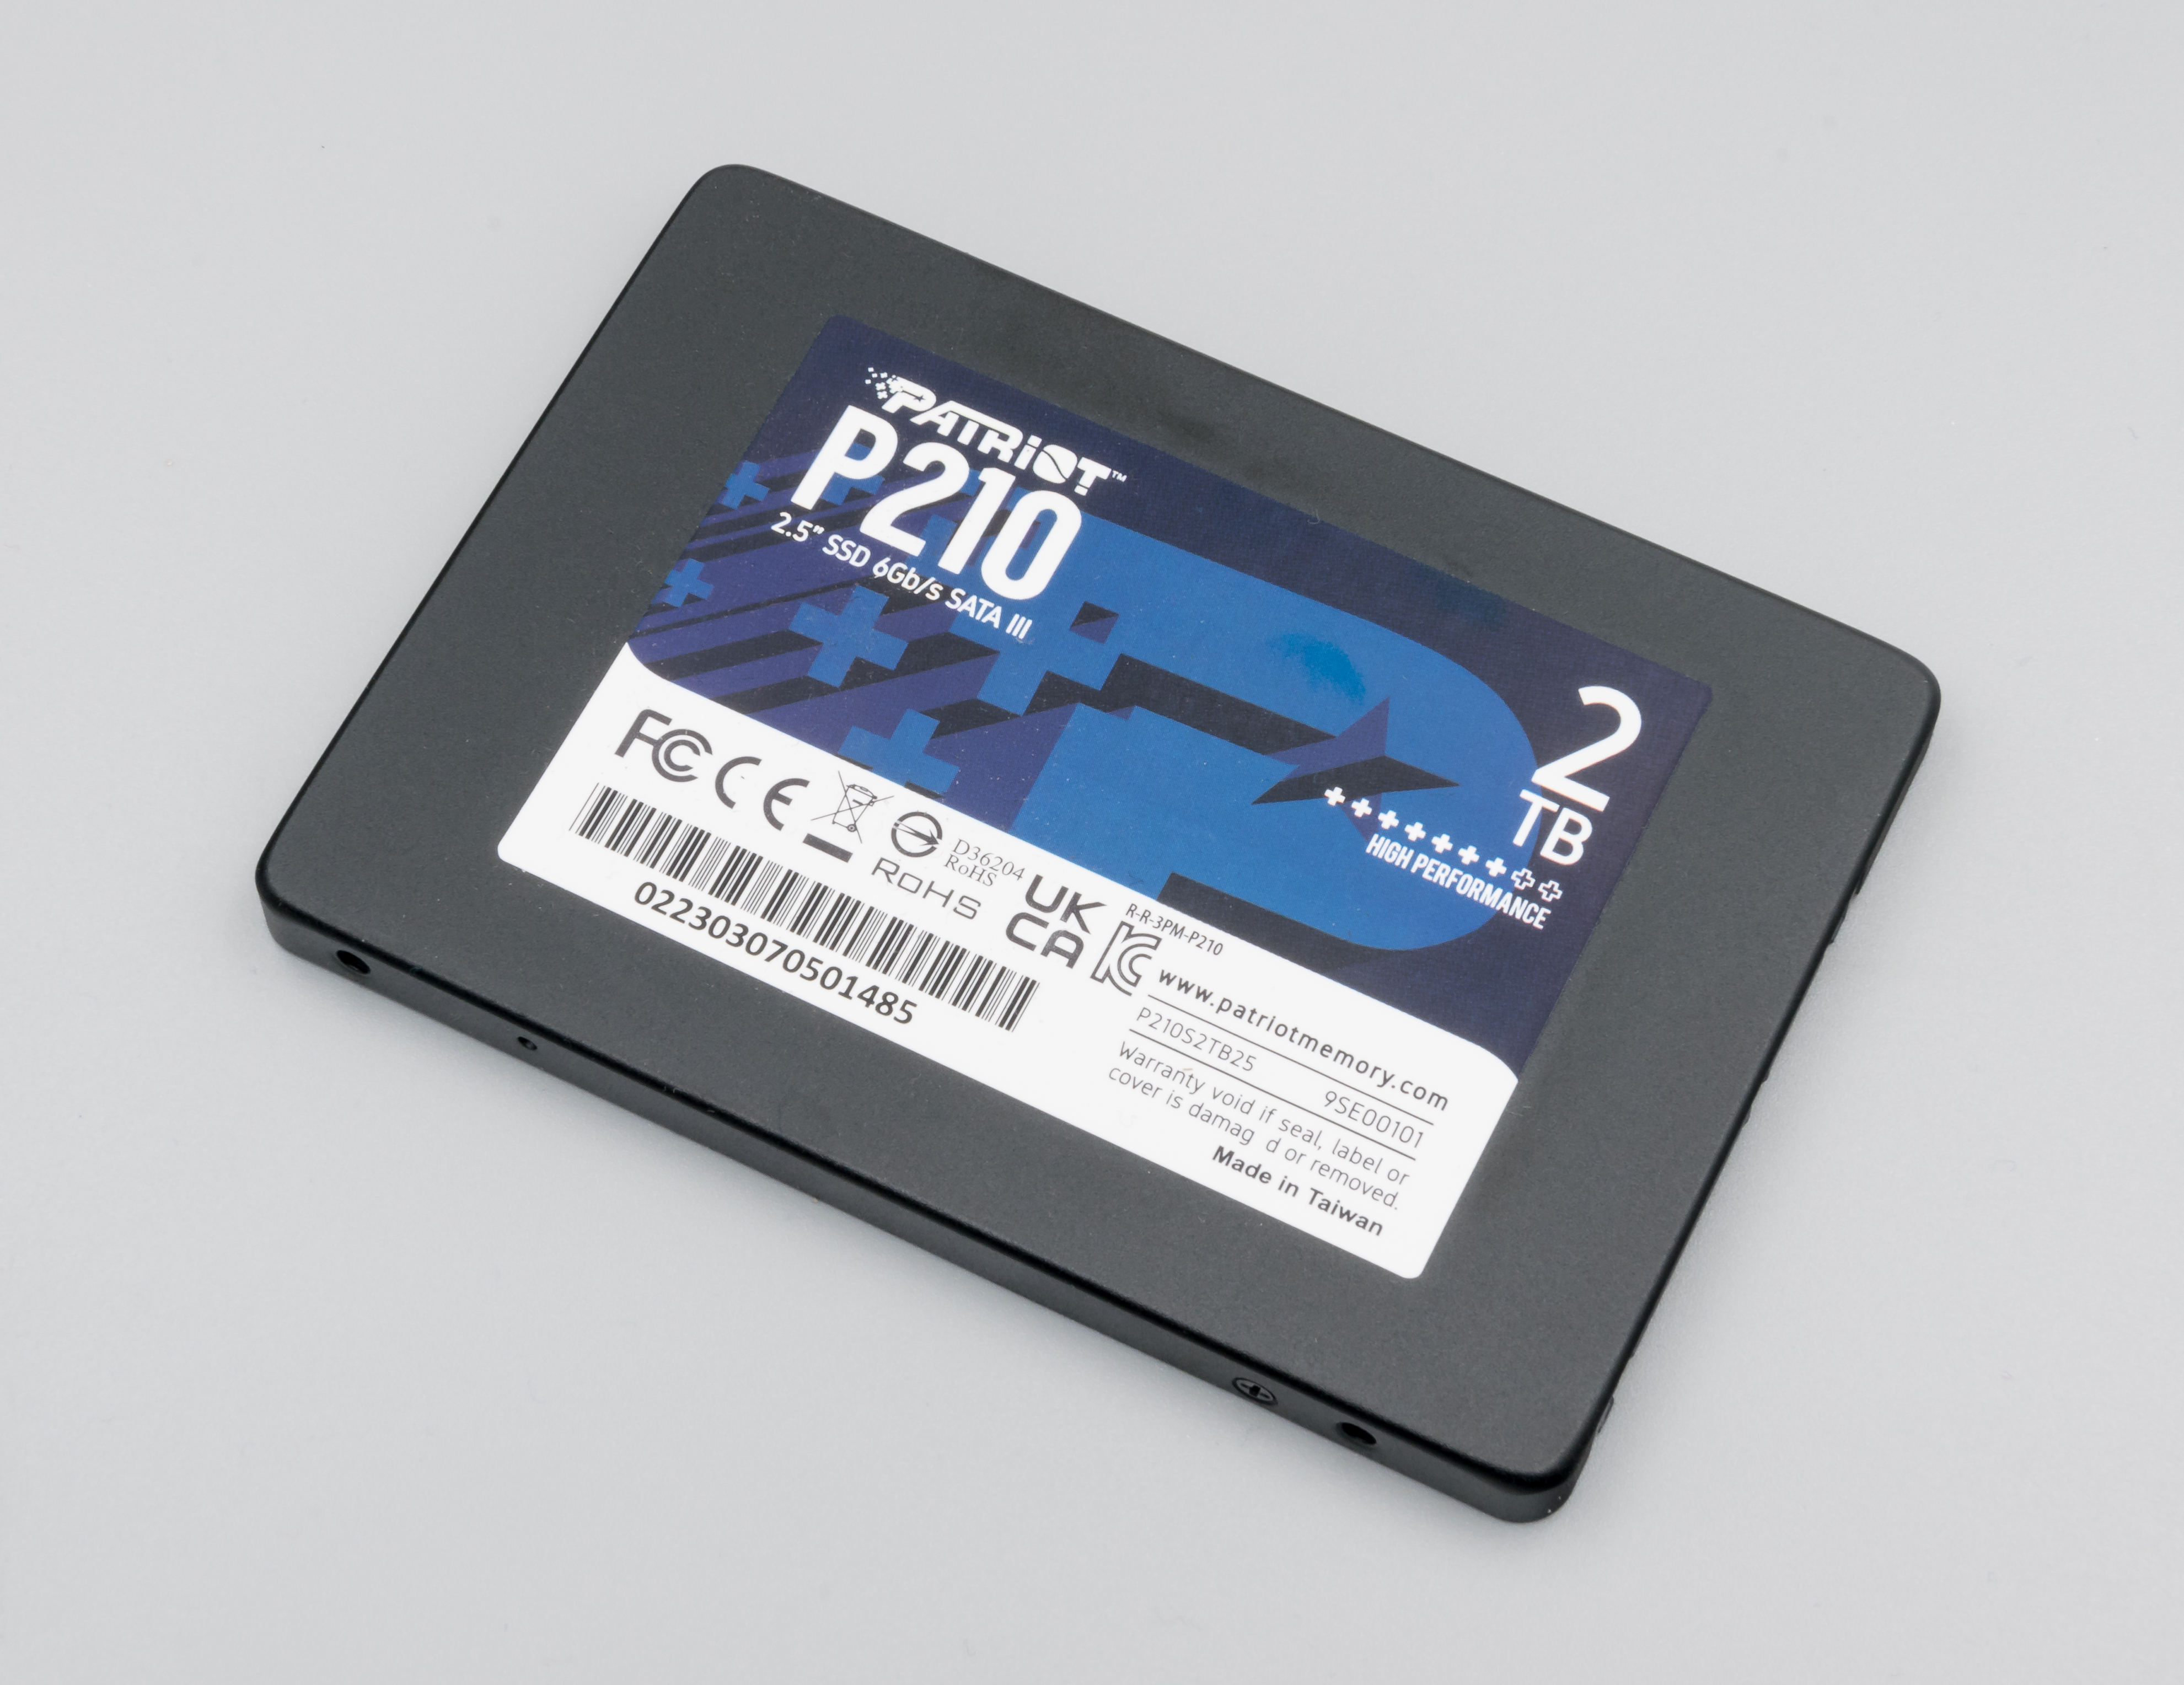
\includegraphics[width=\textwidth,height=\textheight,keepaspectratio]{sdd}
	\item Power supply is like the human heart. It provides power for the whole system just as the heart pumps its blood.
	\includegraphics[width=\textwidth,height=\textheight,keepaspectratio]{power}
	\item Hard disk drive (HDD) is like the long term memory for the humans. It is where the PC stores data that exists in between shutdowns.
	\includegraphics[width=\textwidth,height=\textheight,keepaspectratio]{hdd}
	\item Computer case is like the human brain. It protects the hardware from the environment.
	\includegraphics[width=\textwidth,height=\textheight,keepaspectratio]{chassi}
\end{enumerate}

\section {Task 3}
It was good to refresh my knowledge about computer hardware. 
The ubuntu task was a bit challenging because I failed to do it on my mac with vm ware but it was very easy to setup with virtual box on a windows pc.

\end{document}

% Kan med fördel indelas i underrubriker; Bakgrund, Problemformulering, Litteraturstudie,
% Syfte och mål, Avgränsningar.
%
% Lite skriv-vett
%
% 1. Använd aktiv form (vattnet strömmade genom röret). Det gör rapporten mer livlig.
% 2. Använd dåtid för observationer mm. Exempelvis ”ökat tryck gav större flöde”.
% 3. Använd nutid för generaliseringar och allmänt giltiga påståenden. Exempelvis
% ”I de flesta fall tillhör problemen kategorin olösbara problem”.
% 4. Undvik strunt, pompösa meningar och alla överdrifter. Uttryck som ``utmärkt
% överenstämmelse'' eller ``fantastisk mätnoggrannhet'' får inte förekomma.
% 5. Samtliga tidigare arbeten som åberopas i rapporten skall refereras.
% 6. Skriv inte rapporten som en berättelse om vad ni gjort.
% 7. Berätta inte om de idéer som inte gav något.
% 8. Var mycket försiktig med negativa kommentarer om det egna arbetet.

%%%%%%%%%%%%%%%%%%%%%%%%%%%%%%%%%%%%%%%%%%%%%%%%%%%%%%%%%%%%%%
% -                       Theory                           - %
%%%%%%%%%%%%%%%%%%%%%%%%%%%%%%%%%%%%%%%%%%%%%%%%%%%%%%%%%%%%%%
% \section{Teori}
% Det fysiska lagret syftar till att sköta kommunikationen över det fysiska mediumet.
% Det kan vara exempelvis över wifi eller via en nätverskabel.
% Data länk lagret sköter kommunikationen via en länk, dvs varje två enheter.
% Nätverkslagret sker mellan två enheter, över en eller flera länkar. I detta 
% lager handlar det om att skicka data till rätt host.
% Transportlagret tar hand om datan mellan processorer av två hostar.
% Sessionslagret har hand om en session mellan hostar. Där handlar det 
% om att hålla sessionen uppdaterad.
% Presentationslagret tar hand om kryptering och komprission av data.
% Det sista lagret, applikationslagret, har hand om datan som själva applikationen skall tolka.

% Beskriv teori, antaganden och annat som ligger till grund för den metod och det arbetssätt som valts. Teorin ska belysa/diskutera/sammanfatta och koppla till problemställningen. Samtliga ekvationer, figurer och tabeller ska numreras i löpande ordning. Figurer och tabeller ska ha en kortfattad text som klart och tydligt anger vad de visar. Alla figurer och tabeller ska hänvisas till i löpande text.
% Exempelvis beskrivs en potensfunktion som
% \begin{equation} \label{epotens}
%     y=Cx^k
% \end{equation}
% där exponenten $k$ bestäms genom att logaritmera ekvation (\ref{epotens})
% \begin{equation}
%     \ln y = \ln C + k \ln x \:\:\:\: \Rightarrow \:\:\:\: z = m + kw
% \end{equation}
% $z = \ln y$ plottas mot $w = \ln x$ och lutningen på grafen ger exponenten $k$ ifall mätdata kan beskrivas som en potensfunktion.

% Med figurer avses bilder, diagram, grafer mm. Det ska inte finnas ytterligare rubrik
% i figuren än den som står i figurtexten. Om ej egentillverkad skall källa anges samt
% tillstånd av ägare erhållas.
%
% Variabler skrivs kursivt både i ekvationerna och i brödtexten. Icke-variabler skrivs på vanligt sätt.
% Ekvationer betraktas som en del i texten. Ekvationsnummer ska skrivas längst ut till höger.

% \subsection{Litteraturstudie}

% Måste inte ha egen rubrik utan kan ingå i teorins löpande text.
% I fall teorikapitlet utelämnas ska litteraturstudie ingå i inledningen.

%%%%%%%%%%%%%%%%%%%%%%%%%%%%%%%%%%%%%%%%%%%%%%%%%%%%%%%%%%%%%%
% -                       Method                           - %
%%%%%%%%%%%%%%%%%%%%%%%%%%%%%%%%%%%%%%%%%%%%%%%%%%%%%%%%%%%%%%
% \section{Metod}

% För att initiera TLS behöver slutenheterna komma överens om olika säkerhetsparametrar.
% Därför börjar klienten skicka ett första meddelande som innehåller dessa.
% Men dessa parametrar måste servern och klienten komma överens om. Det kan
% bland annat bero på att en av dem inte stödjer en viss krypteringsalgoritm.
% När samtliga parametrar har bestämts, kan allt därefter vara krypterat med 
% dessa. 


% Kan i vissa fall delas upp i metodbeskrivning, experimentell uppställning och arbetsgång. Att redogöra för sin metod är viktigt bland annat för att förklara varför den valda metoden ger ett tillförlitligt resultat. Alla antaganden och förenklingar måste anges och motiveras. Definiera matematiska modeller så att andra ingenjörer och forskare kan förstå vad du gjort.
% Exempelvis utnyttjades Microsoft Excel 2013 för att analysera mätresultaten och plotta mätdata.

% Här beskrivs metoden, ofta är det lämpligt att dela upp texten i ett antal underrubriker.
% Använd alltid högst tre rubrik-nivåer.

% \subsection{Experimentell uppställning}

% Alla eventuella försöksuppställningar beskrivs på ett sådant sätt att andra kan upprepa samma försök och verifiera dina resultat. Utnyttja figurer som förenklar din beskrivning.

%%%%%%%%%%%%%%%%%%%%%%%%%%%%%%%%%%%%%%%%%%%%%%%%%%%%%%%%%%%%%%
% -                      Results                           - %
%%%%%%%%%%%%%%%%%%%%%%%%%%%%%%%%%%%%%%%%%%%%%%%%%%%%%%%%%%%%%%
% \section{Resultat}

% All kryptering som sker över nätet skall vara rubust och upgraderingsbar. 
% TLS uppfyller detta kriterie.

% Innehåll: resultat och analys.
% I vissa fall kan man ha ”Resultat och diskussion” som kapitel.

% Detta är förmodligen den största delen av rapporten. Här redovisas resultaten rakt på sak på ett objektivt/neutralt sätt. Ofta är det lämpligt att dela upp texten i ett antal underrubriker. Materialet måste presenteras i logisk ordning, vilket inte behöver vara den ordning i vilken försöket/arbetet har utförts.

% Läsaren skall kunna läsa rapporten utan att behöva bläddra fram och tillbaka. Det ska vara tydligt vad som är data respektive analys av data.
% Visas resultat i tabell- eller figurform så måste kortfattat beskrivas vad man ser i figurerna/tabellerna. De placeras i närheten (efter) där de först refererades.

% Som exempel visas fyra mätningar där variabel, 1, varierades. Resultat visas i tabell \ref{tvariabel123} nedan.

% Det skall alltid finnas en tabelltext som förklarar vad som finns i tabellen. Tabellnummer och text ska stå ovanför tabellen.

% \begin{table}[ht]
% \centering
%     \begin{tabular}{c | c | c}
%         \hline
%         variabel 1 (s) & variabel 2 (m) & variabel 3 (J) \\
%         \hline
%         0,351 &	0,693 &	117 \\
%         0,457 &	1,42 &	170 \\
%         0,873 &	2,54 &	300 \\
%         1,10 &	3,21 &	390 \\
%         \hline
%      \end{tabular} 
% \caption{Förklarande text}
% \label{tvariabel123}
% \end{table}

% Med hjälp av mätvärdena i tabell 1 skapas en produktansats av typen potensfunktion
% \begin{equation}
% t = C L^\alpha \theta^\beta m^\gamma g^\delta
% \end{equation}
% där $C, \alpha, ..., \delta$ är konstanter som ska bestämmas experimentellt.
% Avgiven värmemängd från brödrosten (variabel 3) som funktion av tiden variabel 1 visas i figur \ref{fvariabel3vs1}. Den linjära anpassningen i figuren visar att
% \begin{equation}
% {\rm (variabel \, 3)} = 351,8 \cdot {\rm (variabel \, 1)} - 0,3
% \end{equation}
% och tillförd värmeeffekt till brödrosten bestäms då till 351,8 W.

% Diagram ska ha storhet och enhet på axlarna (SI). Är det tex logaritmerade diagram
% ska de ha storhet (men inte enhet) på axlarna. Figurnummer och text ska stå under
% figur och hänga ihop på samma sida.

% \begin{figure}[ht]
% \begin{center}
%   \includegraphics[width=0.6\textwidth]{fig1.png}
%   \caption{Exempelfigur som visar variabel 3 som funktion av variabel 1. \label{fvariabel3vs1}}
% \end{center}
% \end{figure}

% \subsection{Underrubrik vid behov}

% \subsubsection{Fler underrubriker om så behövs}




%%%%%%%%%%%%%%%%%%%%%%%%%%%%%%%%%%%%%%%%%%%%%%%%%%%%%%%%%%%%%%
% -                      Summary                           - %
%%%%%%%%%%%%%%%%%%%%%%%%%%%%%%%%%%%%%%%%%%%%%%%%%%%%%%%%%%%%%%

% \section{Diskussion och slutsatser}

% Kan delas i separata kapitel: ”Diskussion” respektive ”Slutsatser”. Slutsatser skall vara korta och koncisa.
% Ibland är det lämpligast med indelningen ”Diskussion” samt ”Slutsatser och fortsatt arbete”

% Här diskuteras (vad betyder/medför) resultaten utifrån ett vidare perspektiv och ställs i relation exempelvis till tidigare arbeten, referera i sådant fall till dessa. Utgående härifrån dras nödvändiga slutsatser som ska svara på de mål som angivits och vad resultaten har för relevans. Koppla slutsatser till uppställda mål.

% Diskutera felkällor och osäkerheter.
% Det är även lämpligt att i denna del avsluta med förslag och rekommendationer på fortsatta studier och undersökningar i ämnet. Man kan dela upp diskussion, slutsatser och framtida studier i fristående kapitel.




%%%%%%%%%%%%%%%%%%%%%%%%%%%%%%%%%%%%%%%%%%%%%%%%%%%%%%%%%%%%%%
% -                    Bibliography                        - %
%%%%%%%%%%%%%%%%%%%%%%%%%%%%%%%%%%%%%%%%%%%%%%%%%%%%%%%%%%%%%%
\printbibliography % - Here we say that the bibliography should be printed. The section title "References" is printed automatically.

% I denna del anges de källor du använt i ditt arbete. Ange bara de viktigaste och alla
% referenser i listan måste vara refererade till i texten. I referenslistan får det inte
% förekomma någon referens som är ``allmänt bra att ha'' utan endast de referenser som
% författaren själv använt. Alla referenser ska refereras till i texten.
% OBS! använd originalreferenser. Undvik referenser till webbsidor eftersom de kan försvinna/ändras.
% Ett av de vanligaste är att man skriver
% författarnamnet och sedan referensens publikationsår - det s.k. Harvard systemet.
% Exempel: ... även funnet av Charpak (1983)
% Är det två eller flera författare brukar man skriva
% Två författare: ... även funnet av Charpak och Öqvist (1983).
% Flera författare: ... även funnet av Charpak et al. (1983).
% ( et al. är latin (et alii) och betyder ``och andra'').
% Ett annat sätt att ange en referens är att numrera referenserna i den ordning de dyker
% upp i texten och sortera referenslistan i nummerordning.
% Exempel: ... som Öqvist [3] har funnit, och referensen Öqvist dyker då upp som nummer tre i referenslistan.
% En guide för referenser finns här: http://libguides.ltu.se/skrivaoreferera

% \end{document}


